\documentclass[11pt,a4paper,]{article}
\usepackage[]{mathpazo}

\usepackage{amssymb,amsmath}
\usepackage{ifxetex,ifluatex}
\usepackage{fixltx2e} % provides \textsubscript
\ifnum 0\ifxetex 1\fi\ifluatex 1\fi=0 % if pdftex
  \usepackage[T1]{fontenc}
  \usepackage[utf8]{inputenc}
\else % if luatex or xelatex
  \usepackage{unicode-math}
  \defaultfontfeatures{Ligatures=TeX,Scale=MatchLowercase}
\fi
% use upquote if available, for straight quotes in verbatim environments
\IfFileExists{upquote.sty}{\usepackage{upquote}}{}
% use microtype if available
\IfFileExists{microtype.sty}{%
\usepackage[]{microtype}
\UseMicrotypeSet[protrusion]{basicmath} % disable protrusion for tt fonts
}{}
\PassOptionsToPackage{hyphens}{url} % url is loaded by hyperref
\usepackage[unicode=true]{hyperref}
\hypersetup{
            pdftitle={Meta-learning how to forecast time series},
            pdfkeywords={Forecast-model selection, Time series features, Random forest, Algorithm
selection problem, Classsification},
            pdfborder={0 0 0},
            breaklinks=true}
\urlstyle{same}  % don't use monospace font for urls
\usepackage{geometry}
\geometry{a4paper, text={16cm,24cm}}
\usepackage[style=authoryear-comp,]{biblatex}
\addbibresource{FBF.bib}
\usepackage{longtable,booktabs}
% Fix footnotes in tables (requires footnote package)
\IfFileExists{footnote.sty}{\usepackage{footnote}\makesavenoteenv{long table}}{}
\IfFileExists{parskip.sty}{%
\usepackage{parskip}
}{% else
\setlength{\parindent}{0pt}
\setlength{\parskip}{6pt plus 2pt minus 1pt}
}
\setlength{\emergencystretch}{3em}  % prevent overfull lines
\providecommand{\tightlist}{%
  \setlength{\itemsep}{0pt}\setlength{\parskip}{0pt}}
\setcounter{secnumdepth}{5}

% set default figure placement to htbp
\makeatletter
\def\fps@figure{htbp}
\makeatother


\title{Meta-learning how to forecast time series}

%% MONASH STUFF

%% CAPTIONS
\RequirePackage{caption}
\DeclareCaptionStyle{italic}[justification=centering]
 {labelfont={bf},textfont={it},labelsep=colon}
\captionsetup[figure]{style=italic,format=hang,singlelinecheck=true}
\captionsetup[table]{style=italic,format=hang,singlelinecheck=true}

%% FONT
\RequirePackage{bera}
\RequirePackage{mathpazo}

%% HEADERS AND FOOTERS
\RequirePackage{fancyhdr}
\pagestyle{fancy}
\rfoot{\Large\sffamily\raisebox{-0.1cm}{\textbf{\thepage}}}
\makeatletter
\lhead{\textsf{\expandafter{\@title}}}
\makeatother
\rhead{}
\cfoot{}
\setlength{\headheight}{15pt}
\renewcommand{\headrulewidth}{0.4pt}
\renewcommand{\footrulewidth}{0.4pt}
\fancypagestyle{plain}{%
\fancyhf{} % clear all header and footer fields
\fancyfoot[C]{\sffamily\thepage} % except the center
\renewcommand{\headrulewidth}{0pt}
\renewcommand{\footrulewidth}{0pt}}

%% MATHS
\RequirePackage{bm,amsmath}
\allowdisplaybreaks

%% GRAPHICS
\RequirePackage{graphicx}
\setcounter{topnumber}{2}
\setcounter{bottomnumber}{2}
\setcounter{totalnumber}{4}
\renewcommand{\topfraction}{0.85}
\renewcommand{\bottomfraction}{0.85}
\renewcommand{\textfraction}{0.15}
\renewcommand{\floatpagefraction}{0.8}

%\RequirePackage[section]{placeins}

%% SECTION TITLES
\RequirePackage[compact,sf,bf]{titlesec}
\titleformat{\section}[block]
  {\fontsize{15}{17}\bfseries\sffamily}
  {\thesection}
  {0.4em}{}
\titleformat{\subsection}[block]
  {\fontsize{12}{14}\bfseries\sffamily}
  {\thesubsection}
  {0.4em}{}
\titlespacing{\section}{0pt}{*5}{*1}
\titlespacing{\section}{0pt}{*2}{*0.2}


%% TITLE PAGE
\def\Date{\number\day}
\def\Month{\ifcase\month\or
 January\or February\or March\or April\or May\or June\or
 July\or August\or September\or October\or November\or December\fi}
\def\Year{\number\year}

\makeatletter
\def\wp#1{\gdef\@wp{#1}}\def\@wp{??/??}
\def\jel#1{\gdef\@jel{#1}}\def\@jel{??}
\def\showjel{{\large\textsf{\textbf{JEL classification:}}~\@jel}}
\def\nojel{\def\showjel{}}
\def\addresses#1{\gdef\@addresses{#1}}\def\@addresses{??}
\def\cover{{\sffamily\setcounter{page}{0}
        \thispagestyle{empty}%
        \vspace*{-2cm}
        \centerline{\raisebox{-1.8cm}{
\includegraphics[width=5cm]{MBSportrait}}\hspace*{9cm} ISSN 1440-771X}\vspace{0.99cm}
        \begin{center}\Large
        Department of Econometrics and Business Statistics\\[.5cm]
        \scriptsize http://business.monash.edu/econometrics-and-business-statistics/research/publications
        \end{center}\vspace{2cm}
        \begin{center}
        \fbox{\parbox{14cm}{\begin{onehalfspace}\centering\Huge\vspace*{0.3cm}
                \textsf{\textbf{\expandafter{\@title}}}\vspace{1cm}\par
                \LARGE\@author\end{onehalfspace}
        }}
        \end{center}
        \vfill
                \begin{center}\Large
                \Month~\Year\\[1cm]
                Working Paper \@wp
        \end{center}}}
\def\pageone{{\sffamily
        \newpage%\blankpage
        \thispagestyle{empty}
        \vbox to 23cm{
        \raggedright\baselineskip=1.2cm
     {\fontsize{24.88}{30}\sffamily\textbf{\expandafter{\@title}}}
        \vspace{2cm}\par
        \hspace{1cm}\parbox{14cm}{\sffamily\large\@addresses}\vspace{1cm}\vfill
        \hspace{1cm}{\large\Date~\Month~\Year}\\[1cm]
        \hspace{1cm}\showjel\vss}}}
\def\blindtitle{{\sffamily
     \thispagestyle{plain}\raggedright\baselineskip=1.2cm
     {\fontsize{24.88}{30}\sffamily\textbf{\expandafter{\@title}}}\vspace{1cm}\par
        }}
\def\titlepage{{\cover\newpage\setstretch{1}\pageone\newpage\blindtitle}}

\def\blind{\def\titlepage{{\blindtitle}}\let\maketitle\blindtitle}
\def\titlepageonly{\def\titlepage{{\pageone\end{document}}}}
\def\nocover{\def\titlepage{{\newpage\setstretch{1}\pageone\newpage\blindtitle}}\let\maketitle\titlepage}
\let\maketitle\titlepage
\makeatother

%% SPACING
\RequirePackage{setspace}
\spacing{1.5}

%% LINE AND PAGE BREAKING
\sloppy
\clubpenalty = 10000
\widowpenalty = 10000
\brokenpenalty = 10000
\RequirePackage{microtype}

%% PARAGRAPH BREAKS
\setlength{\parskip}{1.4ex}
\setlength{\parindent}{0em}

%% HYPERLINKS
\RequirePackage{xcolor} % Needed for links
\definecolor{darkblue}{rgb}{0,0,.6}
\RequirePackage{url}

\makeatletter
\@ifpackageloaded{hyperref}{}{\RequirePackage{hyperref}}
\makeatother
\hypersetup{
     citecolor=0 0 0,
     breaklinks=true,
     bookmarksopen=true,
     bookmarksnumbered=true,
     linkcolor=darkblue,
     urlcolor=blue,
     citecolor=darkblue,
     colorlinks=true}

%% KEYWORDS
\newenvironment{keywords}{\par\vspace{0.5cm}\noindent{\sffamily\textbf{Keywords:}}}{\vspace{0.25cm}\par\hrule\vspace{0.5cm}\par}

%% ABSTRACT
\renewenvironment{abstract}{\begin{minipage}{\textwidth}\parskip=1.4ex\noindent
\hrule\vspace{0.1cm}\par{\sffamily\textbf{\abstractname}}\newline}
  {\end{minipage}}


\usepackage[T1]{fontenc}
\usepackage[utf8]{inputenc}

\usepackage[showonlyrefs]{mathtools}
\usepackage[no-weekday]{eukdate}

%% BIBLIOGRAPHY

\makeatletter
\@ifpackageloaded{biblatex}{}{\usepackage[style=authoryear-comp, backend=biber, natbib=true]{biblatex}}
\makeatother
\ExecuteBibliographyOptions{bibencoding=utf8,minnames=1,maxnames=3, maxbibnames=99,dashed=false,terseinits=true,giveninits=true,uniquename=false,uniquelist=false,doi=false, isbn=false,url=true,sortcites=false}

\DeclareFieldFormat{url}{\texttt{\url{#1}}}
\DeclareFieldFormat[article]{pages}{#1}
\DeclareFieldFormat[inproceedings]{pages}{\lowercase{pp.}#1}
\DeclareFieldFormat[incollection]{pages}{\lowercase{pp.}#1}
\DeclareFieldFormat[article]{volume}{\mkbibbold{#1}}
\DeclareFieldFormat[article]{number}{\mkbibparens{#1}}
\DeclareFieldFormat[article]{title}{\MakeCapital{#1}}
\DeclareFieldFormat[article]{url}{}
%\DeclareFieldFormat[book]{url}{}
%\DeclareFieldFormat[inbook]{url}{}
%\DeclareFieldFormat[incollection]{url}{}
%\DeclareFieldFormat[inproceedings]{url}{}
\DeclareFieldFormat[inproceedings]{title}{#1}
\DeclareFieldFormat{shorthandwidth}{#1}
%\DeclareFieldFormat{extrayear}{}
% No dot before number of articles
\usepackage{xpatch}
\xpatchbibmacro{volume+number+eid}{\setunit*{\adddot}}{}{}{}
% Remove In: for an article.
\renewbibmacro{in:}{%
  \ifentrytype{article}{}{%
  \printtext{\bibstring{in}\intitlepunct}}}

\AtEveryBibitem{\clearfield{month}}
\AtEveryCitekey{\clearfield{month}}

\makeatletter
\DeclareDelimFormat[cbx@textcite]{nameyeardelim}{\addspace}
\makeatother
\renewcommand*{\finalnamedelim}{%
  %\ifnumgreater{\value{liststop}}{2}{\finalandcomma}{}% there really should be no funny Oxford comma business here
  \addspace\&\space}
  

\wp{??/18}
\jel{C10,C14,C22}


\blind



\date{\sf\Date~\Month~\Year}
\makeatletter
 \lfoot{\sf\@date}
\makeatother

%% Any special functions or other packages can be loaded here.
\usepackage{algorithm}
\usepackage{algpseudocode}
\usepackage{amsthm}
\usepackage{amsmath,bm}
\usepackage{paralist}
\usepackage{todonotes}
\usepackage{ctable}

\def\sectionautorefname{Section}
\captionsetup[figure]{font=small}
\captionsetup[table]{font=small}
\def\var{\text{Var}}
\allowdisplaybreaks
\sloppy

%% LINE AND PAGE BREAKING
\clubpenalty = 4500
\widowpenalty = 4500
\brokenpenalty = 4500


\usepackage{amsthm}
\newtheorem{theorem}{Theorem}[section]
\newtheorem{lemma}{Lemma}[section]
\theoremstyle{definition}
\newtheorem{definition}{Definition}[section]
\newtheorem{corollary}{Corollary}[section]
\newtheorem{proposition}{Proposition}[section]
\theoremstyle{definition}
\newtheorem{example}{Example}[section]
\theoremstyle{definition}
\newtheorem{exercise}{Exercise}[section]
\theoremstyle{remark}
\newtheorem*{remark}{Remark}
\newtheorem*{solution}{Solution}
\begin{document}
\maketitle
\begin{abstract}
A crucial task in time series forecasting is the identification of the
most suitable forecasting method. We present a general framework for
forecast- model selection using meta-learning. A Random Forest is used
to identify the best forecasting method using only time series features.
The proposed framework has been evaluated using time series from the M1
and M3 competitions, and is shown to yield accurate forecasts comparable
to several benchmarks and other commonly used automated approaches of
time series forecasting. A key advantage of our algorithm is that the
time-consuming process of building the random forest can be handled in
advance of the forecasting task.
\end{abstract}
\begin{keywords}
Forecast-model selection, Time series features, Random forest, Algorithm
selection problem, Classsification
\end{keywords}

\setlength{\abovedisplayskip}{5pt} \setlength{\belowdisplayskip}{5pt}
\setlength{\abovedisplayshortskip}{0pt}
\setlength{\belowdisplayshortskip}{0pt}

\section{Introduction}\label{intro}

Forecasting is a key activity for any business to operate efficiently.
The rapid advances in computing technologies have enabled businesses to
keep track of large numbers of time series. Hence, it is becoming
increasingly common to have to regularly forecast many millions of time
series. For example, large scale businesses may be interested in
forecasting sales, cost, and demand for their thousands of products
across different locations, warehouses, etc. Technology companies such
as Google collect many millions of daily time series such as web-click
logs, web search counts, queries, revenues, number of users for
different services, etc., and require fast and accurate automatic
forecasts. However, the scale of these tasks have raised some
computational challenges that we seek to address by proposing a new fast
algorithm for model selection and time series forecasting.

When there is a large number of time series to forecast, there are at
least three possible forecasting strategies: (1) a single method may be
used to provide forecasts across all time series; (2) a framework can be
developed to select the most appropriate forecasting method for each
series; (3) several methods can be applied for each individual series
and the resulting forecasts combined. It is very unlikely that a single
method will consistently outperform its competitors across all time
series, so we reject strategy 1. Because our focus is on fast, scalable
forecasting, we also reject the combination approach (despite it often
being the most accurate of the three strategies), as the computational
requirements are much greater than for strategy 2. We adopt the approach
of selecting an individual forecasting method for each time series to be
forecast.

However, selecting the most appropriate model for a given time series
can also be problematic. Two of the most commonly used automatic
algorithms are the automated Exponential Smoothing Algorithm (ETS) of
\textcite{Hyndman2002} and the automated ARIMA algorithm of
\textcite{Hyndman2008}. Both algorithms are implemented in the forecast
package in R \autocite{forecast}. In this paradigm, a class of models is
selected in advance, and many models within that class are estimated for
each time series. The model with the smallest AICc value is chosen and
used to compute forecasts. This approach relies on the expert judgement
of the forecaster in first selecting the most appropriate class of
models to use, as it is not usually possible to compare AICc values
\emph{between} model classes due to differences in the way the
likelihood is computed, and the way initial conditions are handled.

An alternative approach, which avoids selecting a class of models
\emph{a priori}, is to use a simple ``hold-out'' test set; but then
there is often insufficient data to draw a reliable conclusion. To
overcome this problem, time series cross-validation can be used
\autocite{hyndman2014forecasting}; then models from many different
classes may be applied, and the model with the lowest cross-validated
MSE selected. However, this increases the computation involved
considerably (at least to order \(n^2\) where \(n\) is the number of
series to be forecast).

Clearly, there is a need for a fast, accurate algorithm to automate
forecast-model selection. We propose a general meta-learning framework
using features of the time series to select the class of models, or even
the specific model, to be used for forecasting. The model selection
process is carried out using a classification algorithm --- we use the
time series features as inputs, and the best forecasting algorithm as
the output. The classification algorithm can be built using a large
historical collection of time series, in advance of the real forecasting
exercise (so it is an ``offline'' procedure). Then, when we have a new
time series to forecast, we can quickly compute its features, use the
pre-trained classification algorithm to identify the best forecasting
model, and produce the required forecasts. Thus, the ``online'' part of
our algorithm requires only feature computation, and the application of
a single forecasting model, with no need to estimate large numbers of
models within a class, or to carry out a computationally-intensive
cross-validation procedure.

The rest of this paper is organized as follows. We review the related
work in \autoref{litreview}. In \autoref{methodology} we explain the
detailed components and procedures of our proposed framework for
forecast-model selection. In \autoref{Mcomp} we present the results,
followed by the conclusions and future work in \autoref{discussion}.

\section{Literature Review}\label{litreview}

\subsection{Time series features}\label{time-series-features}

Rather than work with the time series directly at the level of
individual observations, we propose analysing time series via an
associated ``feature space''. A time series feature is any measurable
characteristic of a time series. For example, \autoref{fig:fig1} shows
the time-domain representation of six time series taken from the M3
competition \autocite{makridakis2000m3} while \autoref{fig:fig2} shows a
feature-based representation of the same time series. Here only two
features are considered: the strength of seasonality and the strength of
trend, calculated based on the measures introduced by
\textcite{wang2009rule}. Time series in the lower right quadrant of
\autoref{fig:fig2} are non-seasonal but trended, while there is only one
series with both high trend and high seasonality. We also see how the
degree of seasonality and trend varies between series. Other examples of
time series features include autocorrelation, spectral entropy and
measures of self-similarity and non-linearity.
\textcite{fulcher2014highly} introduced 9000 operations to extract
features from time series.

\begin{figure}

{\centering 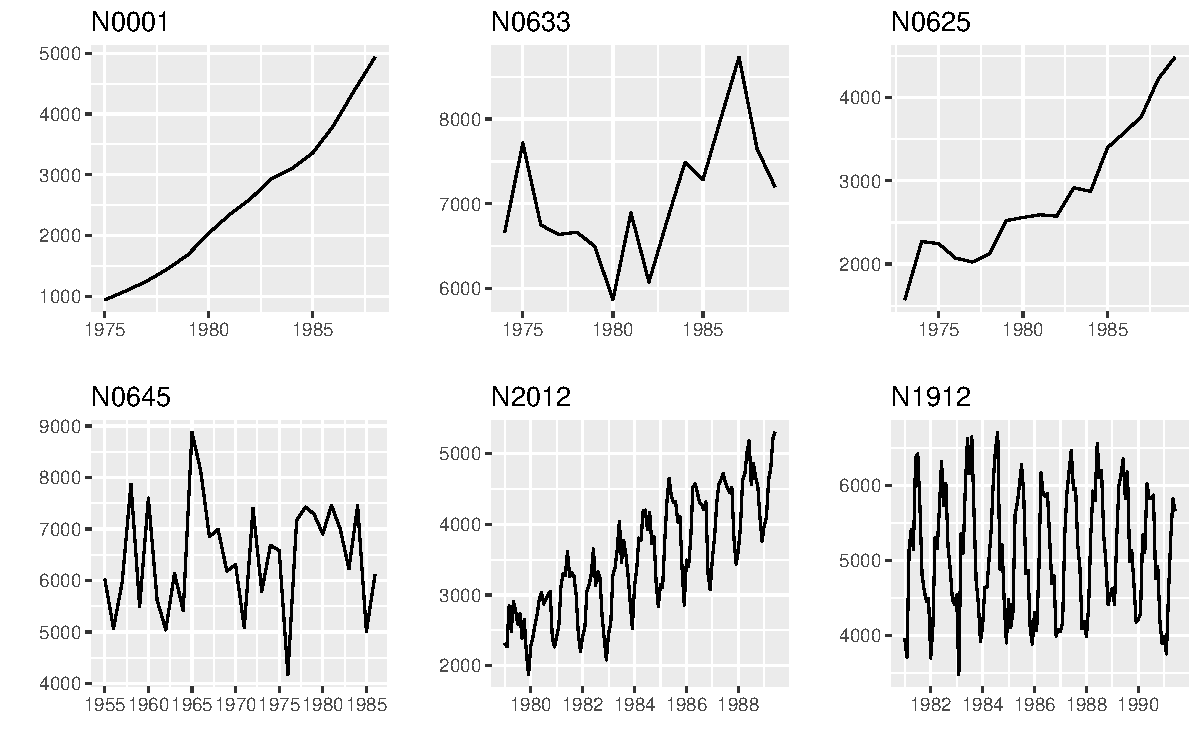
\includegraphics[width=\textwidth]{figure/fig1-1} 

}

\caption{Time-domain representation of time series}\label{fig:fig1}
\end{figure}

\begin{figure}

{\centering 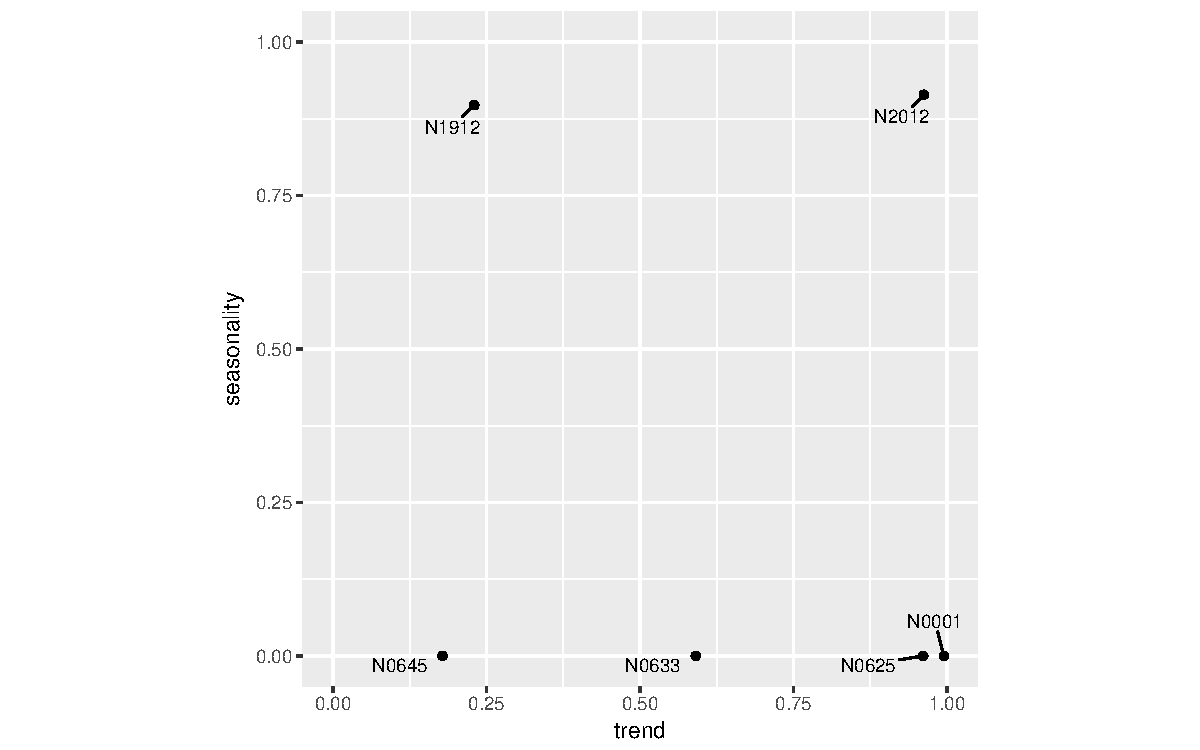
\includegraphics[width=0.7\linewidth]{figure/fig2-1} 

}

\caption{Feature-based representation of time series}\label{fig:fig2}
\end{figure}

The choice of the most appropriate set of features depends on both the
nature of the time series being analysed, and the purpose of the
analysis. In \autoref{Mcomp}, we study time series that have been used
in the M1 and M3 competitions
\autocites{makridakis1982accuracy}{makridakis2000m3}, and we select time
series features for the purpose of forecast-model selection. Because the
M1 and M3 competitions involve time series of different lengths, on
different scales, and with different properties, we restrict our
features to be ergodic, stationary and independent of scale. Because we
are concerned with forecasting, we select features which have
discriminatory power in selecting a good model for forecasting.

\subsection{What makes features useful for forecast-model
selection?}\label{what-makes-features-useful-for-forecast-model-selection}

\textcite{reid1972comparison} pointed out that the performance of
forecasting methods changes according to the nature of the data, and if
the reasons for these variations are explored, they may be useful in
selecting the most appropriate model. In response to the results of the
M3 competition \autocite{makridakis2000m3}, similar ideas have been
reported by others, who have argued that the characteristics of various
time series may provide useful insights into which forecasting methods
are most appropriate to forecast a given time series
\autocites{hyndman2001s}{lawrence2001s}{armstrong2001s}.

Many time series forecasting techniques have been developed to capture
specific characteristics of time series that are common in a particular
discipline. For example, GARCH models were introduced to account for
time-varying volatility in financial time series, and ETS models were
introduced to handle the trend and seasonal patterns which are typical
in quarterly and monthly sales data. An appropriate set of features
should reveal the characteristics of the time series that are useful in
determining the best forecasting method.

Several researchers have introduced rules for forecasting based on
features \autocites{collopy1992rule}{adya2001automatic}{wang2009rule}.
\textcite{kang2017visualising} applied principal component analysis to
project a large collection of time series into a two dimensional feature
space in order to visualize what makes a particular forecasting method
perform well or not. The features they considered were spectral entropy,
first-order auto-correlation coefficient, strength of trend, strength of
seasonality, seasonal period and optimal Box-Cox transformation
parameter. They also proposed a method for generating new time series
based on specified features.

\subsection{Meta-learning for algorithm
selection}\label{meta-learning-for-algorithm-selection}

John Rice was an early and strong proponent of the idea of
meta-learning, which he called the algorithm selection problem (ASP)
\autocite{rice1976}. The term \emph{meta-learning} started to appear
with the emergence of the machine-learning literature. Rice's framework
for algorithm selection is shown in \autoref{fig:rice}.

\begin{figure}

{\centering 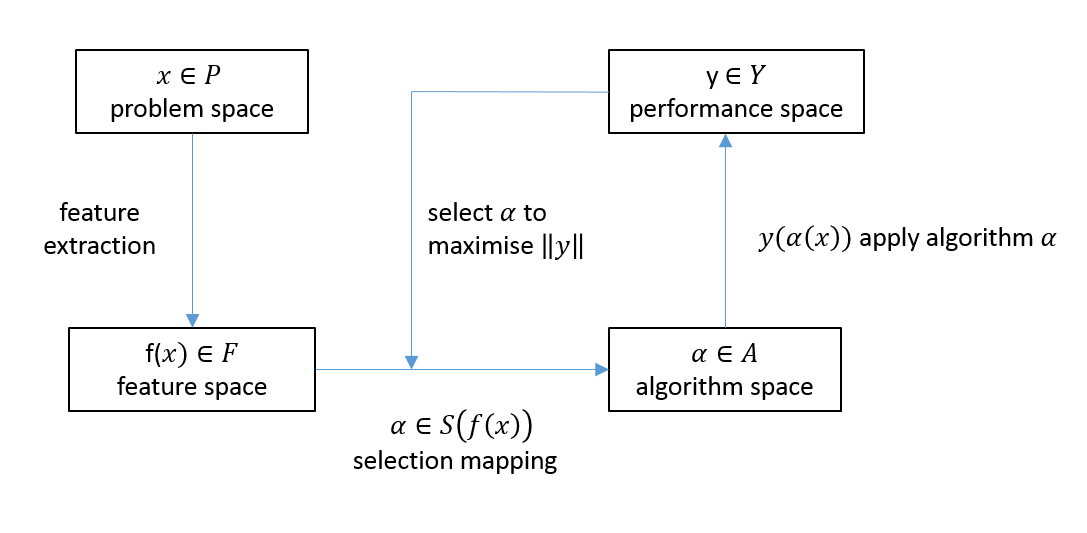
\includegraphics[width=0.8\linewidth]{figures/RiceFramework} 

}

\caption{Rice's framework for the Algorithm Selection Problem (reproduced from Smith-Miles, 2009)}\label{fig:rice}
\end{figure}

There are four main components in Rice's framework. The problem space,
\(P\), represents the data sets used in the study. The feature space,
\(F\), is the range of measures that characterize the problem space
\(P\). The algorithm space, \(A\), is a list of suitable candidate
algorithms which we can use to find solutions to the problems in \(P\).
The performance metric, \(Y\), is a measure of algorithm performance
such as accuracy, speed, etc. Rice's formal definition of the algorithm
selection problem is \autocite{smith2009cross} as follows.

\begin{definition}
\label{def2}
For a given problem instance $x \in P$, with features $f(x) \in F$, find the selection mapping $S(f(x))$ into algorithm space $A$, such that the selected algorithm $\alpha \in A$ maximizes the performance mapping $y(\alpha(x)) \in Y$.
\end{definition}

The main challenge in ASP is to identify the selection mapping \(S\)
from the feature space to the algorithm space. Even though Rice's
framework articulates a conceptually rich framework, it does not specify
how to obtain \(S\). This gives rise to the meta-learning approach.

The meta-learning framework consists of an offline (training) phase and
an online (prediction) phase. In the offline phase, the mapping \(S\) is
learned based on a collection of training examples. This is performed
using a \emph{meta-learner} which can be any supervised learning
algorithm designed to estimate \(S\). The inputs for the meta-learner
are known as \emph{meta-features}, and instances in the algorithm space
are the \emph{output labels}. The database comprising both
input-features and output-labels is called \emph{meta-data}. In the
online phase of the algorithm, input-features are extracted from new
data and passed into the meta-learner that was constructed in the
offline phase, in order to predict the output-labels of the new data.

\subsection{Forecast-model selection using
meta-learning}\label{forecast-model-selection-using-meta-learning}

Selecting models for forecasting can be framed according to Rice's ASP
framework.

\begin{definition}
\label{def2}
For a given time series $x \in P$, with features $f(x) \in F$, find the selection mapping $S(f(x))$ into the algorithm space $A$, such that the selected algorithm $\alpha \in A$ minimizes forecast accuracy error metric $y(\alpha(x)) \in Y$ on the test set of the time series.
\end{definition}

Existing methods differ with respect to the way they define the problem
space (\(A\)), the features (\(F\)), the forecasting accuracy measure
(\(Y\)) and the selection mapping (\(S\)).

\textcite{collopy1992rule} introduced 99 rules based on 18 features of
time series, in order to make forecasts for economic and demographic
time series. This work was extended by \textcite{armstrong2001s} to
reduce human intervention. \textcite{shah1997model} used the following
features to classify time series: the number of observations, the ratio
of the number of turning points to the length of the series, the ratio
of number of step changes, skewness, kurtosis, the coefficient of
variation, autocorrelations at lags 1--4, and partial autocorrelations
at lag 2--4. Casting Shah's work in Rice's framework, we can specify:
\(P=203\) quarterly series from the M1 competition
\autocite{makridakis1982accuracy}; \(A=3\) forecast-models, namely
simple exponential smoothing, Holt-Winters exponential smoothing with
multiplicative seasonality, and a basic structural time series model;
\(Y=\) mean squared error for a hold-out sample. The mapping \(S\) is
learned using discriminant analysis.

\textcite{prudencio2004meta} was the first paper to use the term
``meta-learning'' in the context of time series model selection. They
studied the applicability of meta-learning approaches for forecast-model
selection based on two case studies. Again using the notation of
Definition \ref{def2}, we can describe their first case study with:
\(A\) contained only two forecast-models, simple exponential smoothing
and a time-delay neural network; \(Y=\) mean absolute error; \(F\)
consisted of 14 features, namely length, autocorrelation coefficients,
coefficient of variation, skewness, kurtosis, and a test of turning
points to measure the randomness of the time series; \(S\) was learnt
using the C4.5 decision tree algorithm. For their second study, the
algorithm space included a random walk, Holt's linear exponential
smoothing and AR models; the problem space \(P\) contained the yearly
series from the M3 competition \autocite{makridakis2000m3}; \(F\)
included a subset of features from the first study; and \(Y\) was a
ranking based on error. Beyond the task of forecast-model selection,
they used the NOEMON approach to rank the algorithms
\autocite{kalousis1999noemon}.

\textcite{lemke2010meta} studied the applicability of different
meta-learning approaches for forecast-model selection. Their algorithm
space \(A\) contained ARIMA models, exponential smoothing models and a
neural network model. In addition to statistical measures such as the
standard deviation of the detrended series, skewness, kurtosis, length,
strength of trend, Durbin-Watson statistics of regression residuals, the
number of turning points, step changes, a predictability measure,
nonlinearity, the largest Lyapunov exponent, and auto-correlation and
partial-autocorrelation coefficients, he also used frequency domain
based features. The feed forward neural network, decision tree and
support vector machine approaches were considered to learn the mapping
\(S\).

\textcite{wang2009rule} used a meta-learning framework to provide
recommendations as to which forecast method to use to generate
forecasts. In order to evaluate forecast accuracy, they introduced a new
measure \(Y =\) \emph{simple percentage better (SPB)}, which calculates
the forecasting accuracy of a method against the forecasting accuracy
error of random walk model. They used a feature set \(F\) comprising
nine features: strength of trend, strength of seasonality, serial
correlation, nonlinearity, skewness, kurtosis, self-similarity, chaos
and periodicity. The algorithm space \(A\) included eight
forecast-models, namely, exponential smoothing, ARIMA, neural networks
and random walk model; while the mapping \(S\) was learned using the
C4.5 algorithm for building decision trees. In addition, they used SOM
clustering on the features of the time series in order to understand the
nature of time series in a two-dimensional setting.

The set of features introduced by \textcite{wang2009rule} was later used
by \textcite{widodomodel} to develop a meta-learning framework for
forecast-model selection. The authors further reduced the dimensionality
of time series by performing principal component analysis on the
features.

More recently, \textcite{kuck2016meta} proposed a meta-learning
framework based on neural networks for forecast-model selection. Here,
\(P = 78\) time series from the NN3 competition were used to build the
meta-learner. They introduced a new set of features based on forecasting
errors. The average symmetric mean absolute percentage error was used to
identify the best forecast-models for each series. They classify their
forecast-models in the algorithm space \(A\), comprising single,
seasonal, seasonal-trend and trend exponential smoothing. The mapping
\(S\) was learned using a feed-forward neural network. Further, they
evaluated the performance of different sets of features for
forecast-model selection.

\section{Methodology}\label{methodology}

Our proposed framework is presented in \autoref{fig:framework}. The
offline and online parts of the framework are shown in blue and red
respectively. A classification algorithm (the meta-learner) is trained
during the offline phase and then is used to select appropriate
forecast-models for new time series in the online phase.

\begin{figure}

{\centering 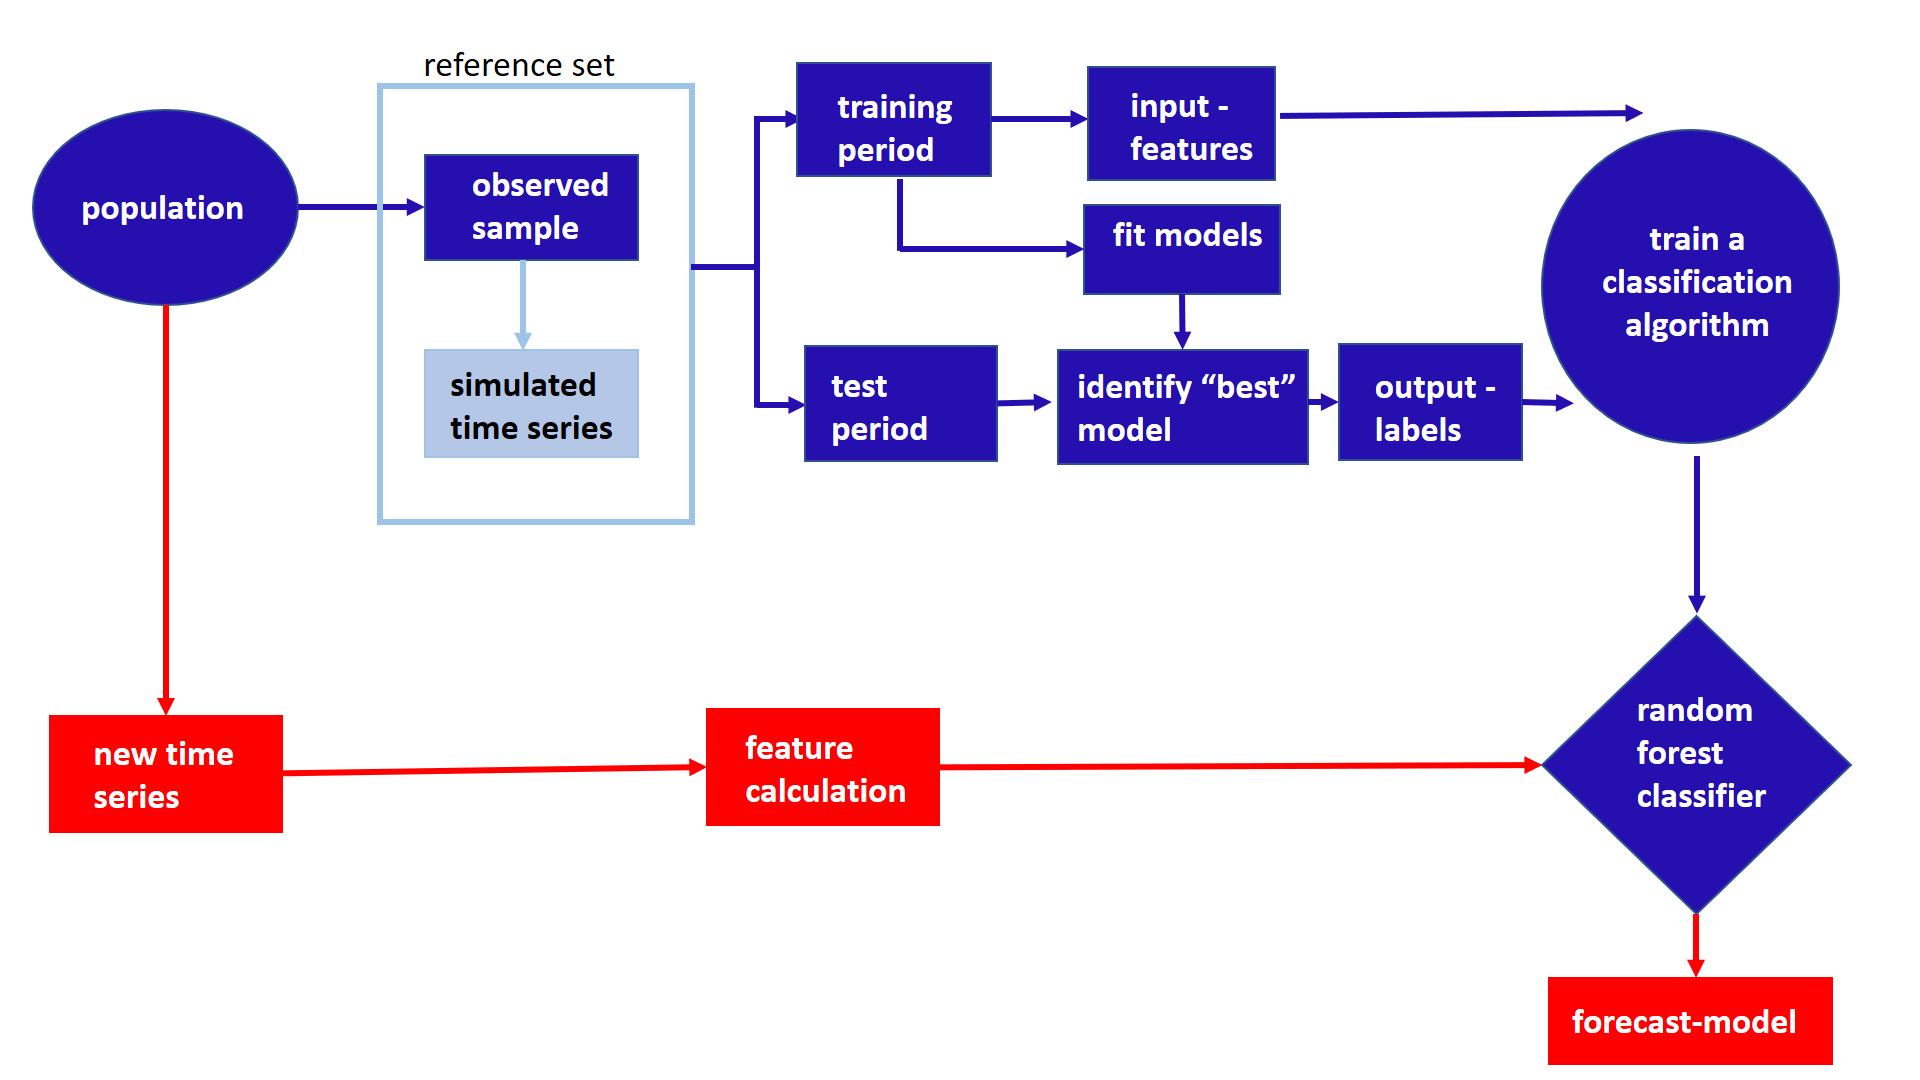
\includegraphics[width=\textwidth]{figures/framework} 

}

\caption{Proposed framework (blue: offline phase, red: online phase)}\label{fig:framework}
\end{figure}

\begin{algorithm}[!hb]
  \caption{Identification of the "best" forecast method for a new time series.}
  \label{alg:algo-lab}
  \begin{algorithmic}[1]
    \Statex \textbf{Offline phase}
    \Statex \text{Given:}
    \Statex \hspace{1cm}$O=\{t_1, t_2, \dots,t_n\}:$ the collection of $n$ observed time series.
      \Statex \hspace{1cm}$L:$ the set of class labels (e.g.\ ARIMA, ETS, SNAIVE).
         \Statex \hspace{1cm}$F:$ the set of functions to calculate time series features.
         \Statex \hspace{1cm}$nsim:$ number of series to be simulated.
         \Statex \hspace{1cm}$B:$ number of trees in the random forest.
         \Statex \hspace{1cm}$mtry:$ number of features to be selected at each node.
     \Statex \text{Output:}
      \Statex \hspace{1cm}\text{a random forest classifier} 
      \Statex
     \Statex \textit{Prepare the reference set}
    \Statex For $i=1$ to $n$:
            \State Fit ARIMA and ETS models to $t_i$.
            \State Simulate $nsim$ time series from each model in step 1.
            \State The time series in $O$ and simulated time series in step 2 form the reference set $R=\{t_1, t_2, \dots,t_n, t_{n+1},\dots,t_N\}$ where $N = n + nsim$.
    \Statex 
    \Statex \textit{Prepare the meta-data}
    \Statex For $j=1$ to $N$:
            \State Split $t_j$ into a training period and test period.
            \State Calculate features $F$ based on the training period. 
            \State Fit $L$ models to the training period.
            \State Calculate forecasts for the test period from each model.
            \State Calculate forecast error measure over the test period for all models in $L$.
            \State Select the model with the minimum forecast error.
            \State Meta-data: input features (step 5), output labels (step 9).
     \Statex
    \Statex \textit{Train a random forest classifier}
            \State Train a random forest classifier based on the meta-data.
            \State {Random forest: the ensemble of trees $\{T_b\}_1^B$}. 
    \Statex
     \Statex \textbf{Online phase}
    \Statex \text{Given:}
    \Statex \hspace{1cm}\text{the random forest classifier from step 12} .
     \Statex \text{Output:}
      \Statex \hspace{1cm}\text{class labels for newly arrived time series $t_{new}$}.
  \State For $t_{new}$ calculate features $F$.
  \State Let $\hat{C_b}(t_{new})$ be the class prediction of the $b^{th}$ random forest tree. Then class label for $t_{new}$ is $\hat{C_{rf}}(t_{new})=majorityvote\{\hat{C_b}(t_{new})\}_1^B$.
   \end{algorithmic}
\end{algorithm}

In order to train our classification algorithm, we need a large
collection of time series which are similar to those we will be
forecasting. We assume that we have an essentially infinite population
of time series, and we take a sample of them in order to train the
classification algorithm. The new time series we wish to forecast can be
thought of as additional draws from the same population. Hence, any
conclusions made from the classification framework refer only to the
population from which the sample has been selected. We may call this the
``target population'' of time series. It is important to have a
well-defined target population to avoid misapplying the classification
rules. We denote the collection of time series used for training the
classifier as the ``reference set''. We split each time series within
the reference set into a training period and a test period. From each
training period we compute a range of time series features, and fit a
selection of potential models. The calculated features form the input
vector to the classification algorithm. Using the fitted models, we
generate forecasts and identify the ``best'' model for each time series
based on a forecast error measure (e.g., MASE) calculated over the test
period. The models deemed ``best'' form the output labels for the
classification algorithm. The pseudo code for this algorithm is given in
Algorithm \autoref{alg:algo-lab}. In the following sections, we briefly
discuss aspects of the offline part of the algorithm.

\subsection{Augmenting the observed sample with simulated
series}\label{augmenting-the-observed-sample-with-simulated-series}

In practice, we may wish to augment our set of training time series by
simulating new time series that are similar to those from the
population. This process may be useful when our observed sample of time
series is too small to build a reliable classifier. Alternatively, we
may wish to add more of some types of time series to the reference set
in order to get a more balanced sample for the classification. In order
to produce simulated series that are similar to our population, we
consider two classes of data generating processes: Exponential Smoothing
Models and ARIMA models using automated algorithms such as \texttt{ets}
and \texttt{auto.arima} \autocite{forecast}. We identify models, based
on model selection criteria (such as AICc) and simulate multiple time
series from the selected models within each model class. Assuming the
models produce data that are similar to the observed time series, this
ensures that the simulated series are similar to those in the
population. Note that this is done in the offline phase of the
algorithm, so the computational time in producing these simulated series
is of no real consequence.

\subsection{Input: features}\label{input-features}

Our proposed algorithm requires features that enable identification of a
suitable forecast-model for a given time series. Therefore, the features
used should capture the dynamic structure of the time series, such as
autocorrelation, trend, seasonality, nonlinearity, heterogeneity, and so
on.

The purpose of this feature-based framework is to reduce the time
required for model selection. Therefore, time needed to calculate the
input features should be significantly less than the time required to
estimate the parameters of all candidate models in a model selection
procedure. Furthermore, interpretability, robustness to outliers, scale
and length independence need to be considered when selecting features
for this classification problem. A comprehensive description of the
features used in the experiment is specified in \autoref{feature}.

\subsection{Output: labels}\label{output-labels}

The task of our classification framework is to identify the best
forecasting method for a given time series. We define the best
forecasting method as the model with the lowest forecast accuracy
measure (e.g., MAPE or MASE) over the test period.

It is not possible to train all possible classes of time series models.
At the very least we should consider enough possibilities so that the
algorithm can be used for model selection with high confidence. The
models considered will depend on the specific population of time series
we need to forecast. For example, if we have only non-seasonal time
series, and no chaotic features, we may wish to restrict our models to
random walks, white noise, ARIMA processes and ETS processes. Even in
this scenario, the number of possible models can be quite large. In
order to identify the best forecasting method for each series, all the
models considered are run on all time series in the reference set, and
forecasts are generated from each of them. Model estimation is strictly
done on the training period of each series and forecasts are compared
with the values in the test period. This step is computationally
intensive and time-consuming, as all models have to be applied on each
series in the reference set. However, since this is done only in the
offline phase, the time involved and the computational cost associated
with this task is of no significant cost.

\subsection{Random forest algorithm}\label{random-forest-algorithm}

A random forest \autocite{breiman2001random} is an ensemble learning
method that combines a large number of decision trees using a two-step
randomization process. Let
\(Z=\{(\bm{x}_1, y_1), (\bm{x}_2, y_2), \dots, (\bm{x}_N, y_N)\}\) be
the reference set, where the input \(\bm{x}_i\) is an \(m\)-vector of
features, the output, \(y_i\), corresponds to the class label of the
\(i\)th observation, \(m\) is the total number of features, and \(N\) is
the number of training samples in the reference set. Each tree in the
forest is grown based on a bootstrap sample of size \(N\) from the
reference set. At each node of the tree, randomly select \(f<m\)
features from the full set of features. The best split is selected among
those \(f\) features. The split which results in the most homogeneous
subnodes is considered the best split. Various measures have been
introduced to evaluate the homogeneity of subnodes, such as
classification error rate, the Gini index and cross entropy
\autocite{friedman2001elements}. In this study, we use the Gini index to
evaluate the homogeneity of a particular split. The trees are grown to
the largest extent possible without pruning. To determine the class
label for a new instance, features are calculated and passed down the
trees. Then each tree gives a prediction and the majority vote over all
individual trees leads to the final decision. In this work, we have used
the randomForest package \autocites{liaw2002randomforest}[;][]{rfpkg} in
R \autocite{Rcore} which implements the Fortran code for Random Forest
classification by \textcite{breiman2004random}.

\section{Application to M competition Data}\label{Mcomp}

To test how well our proposed framework can identify suitable
forecast-models, we use the time series of the M1 competition
\autocite{makridakis1982accuracy} and M3 competition
\autocite{makridakis2000m3}. The R package Mcomp \autocite{hyndmanmcomp}
provides the data from both competitions. The proposed algorithm is
applied to yearly, quarterly and monthly series separately. We run two
experiments for each case. In the first experiment, we treat the time
series of the M1 competition as the \emph{observed sample} and the time
series of the M3 competition as the collection of \emph{new time
series}. We reverse the sets in the second experiment, using the M3 data
as the \emph{observed sample} and the M1 data as the \emph{new time
series}. This allow us to compare our results with published forecast
accuracy results for each competition. In both experiments, we fit ARIMA
and ETS models to the full length of each series in the corresponding
\emph{observed samples} using the \texttt{auto.arima} and \texttt{ets}
functions in the forecast package \autocite{forecast}. From each model
fitted to annual and quarterly data, we simulate a further 1000 series.
For monthly time series, we simulate a further 100 series (to speed up
the offline calculation process). The lengths of the simulated time
series are set to be equal to the lengths of the series on which they
were based.

As shown in \autoref{fig:framework}, the task of constructing the
meta-database contains two main components: (i) identification of an
\emph{output-label} and (ii) computation of features.

The output-labels we consider in this experiment are:

\begin{compactenum}[\hspace*{1cm}(a)]
  \item White noise process (WN);
  \item AR/ MA/ ARMA;
  \item ARIMA;
  \item Random walk with drift (RWD);
  \item Random walk (RW);
  \item Theta;
  \item STL-AR;
  \item Exponential Smoothing Model (ETS) without trend and seasonal components;
  \item ETS with trend component and without seasonal component;
  \item ETS with damped trend component and without seasonal component;
  \end{compactenum}

Most of these are self-explanatory labels based on models implemented in
the forecast package \autocite{forecast}. STL-AR refers to a model based
on an STL decomposition method applied to the time series, then an AR
model is used to forecast the seasonally adjusted data, while the
seasonal naive method is used to forecast the seasonal component.

In addition to the above ten output labels, we further include the
following five class labels for seasonal data:

\begin{compactenum}[\hspace*{1cm}(a)]\setcounter{enumi}{10}
  \item ETS with trend and seasonal components
  \item ETS with damped trend and seasonal components
  \item ETS with seasonal components and without trend component
  \item SARIMA
  \item Seasonal naive method.
  \end{compactenum}

The models are estimated using the training period for each series, and
forecasts are produced for the whole of the test periods. We further use
the \texttt{auto.arima} and \texttt{ets} functions in the forecast
package to identify suitable AR/MA/ARMA, ARIMA, SARIMA and ETS models.
The model corresponding to the smallest MASE
\autocite{hyndman2006another} for the test period is selected as the
\emph{output-label}.

\subsection{Feature computation process}\label{sec:features}

We use a set of 25 features for yearly data and a set of 30 features for
seasonal data. Some of these are taken from previous studies
\autocites{wang2009rule}{hyndman2015large}{kang2017visualising}, and we
have added some new features that we believe provide some useful
information. Each feature can be computed rapidly, thus making the
online phase of our algorithm very fast. The features are summarized in
\autoref{feature}, and fully described in the Appendix.

\begin{table}[!htp]
\centering\footnotesize\tabcolsep=0.12cm
\def\yes{$\checkmark$}
\caption{Features used for selecting a forecast-model.}
\label{feature}
\begin{tabular}{llp{8,8cm}cc}
\toprule
\multicolumn{2}{c}{Feature} & Description & Non-seasonal & Seasonal\\ 
\midrule
1  & T              & length of time series                                                                   & \yes  & \yes \\
2  & trend          & strength of trend                                                                       & \yes  & \yes\\
3  & seasonality       & strength of seasonality                                                                 & -     & \yes \\
4  & linearity      & linearity                                                                               & \yes  & \yes \\
5  & curvature      & curvature                                                                               & \yes  & \yes \\
6  & spikiness      & spikiness                                                                               & \yes  & \yes \\
7  & e\_acf1        & first ACF value of remainder series                                                     & \yes  & \yes \\
8  & stability      & stability                                                                               & \yes  & \yes \\
9  & lumpiness      & lumpiness                                                                               & \yes  & \yes \\
10 & entropy        & spectral entropy                                                                        & \yes  & \yes \\
11 & hurst          & Hurst exponent                                                                          & \yes  & \yes \\
12 & nonlinearity   & nonlinearity                                                                            & \yes\ & \yes \\
13 & alpha          & ETS(A,A,N) $\hat\alpha$                                                                 & \yes  & \yes \\
14 & beta           & ETS(A,A,N) $\hat\beta$                                                                  & \yes  & \yes\\
15 & hwalpha        & ETS(A,A,A) $\hat\alpha$                                                                 & -     & \yes \\
16 & hwbeta         & ETS(A,A,A) $\hat\beta$                                                                  & -     & \yes \\
17 & hwgamma        & ETS(A,A,A) $\hat\gamma$                                                                 & -     & \yes \\
18 & ur\_pp         & test statistic based on Phillips-Perron test                                            & \yes  & - \\
19 & ur\_kpss       & test statistic based on KPSS test                                                       & \yes  & - \\
20 & y\_acf1        & first ACF value of the original series                                                  & \yes  & \yes \\
21 & diff1y\_acf1   & first ACF value of the differenced series                                               & \yes  & \yes \\
22 & diff2y\_acf1   & first ACF value of the twice-differenced series                                         & \yes  & \yes \\
23 & y\_acf5        & sum of squares of first 5 ACF values of original series                                 & \yes  & \yes \\
24 & diff1y\_acf5   & sum of squares of first 5 ACF values of differenced series                              & \yes  & \yes \\
25 & diff2y\_acf5   & sum of squares of first 5 ACF values of twice-differenced series                        & \yes  & \yes \\
26 & seas\_acf1     & autocorrelation coefficient at first seasonal lag                                                & -     & \yes \\
27 & sediff\_acf1   & first ACF value of seasonally-differenced series                                        & -     & \yes\\
28 & sediff\_seacf1 & ACF value at the first seasonal lag of seasonally-differenced series                    & -     & \yes \\
29 & sediff\_acf5   & sum of squares of first 5 autocorrelation coefficients of seasonally-differenced series & -     & \yes \\
30 & lmres\_acf1    & first ACF value of residual series of linear trend model                                & \yes  & - \\
31 & y\_pacf5       & sum of squares of first 5 PACF values of original series                                & \yes  & \yes \\
32 & diff1y\_pacf5  & sum of squares of first 5 PACF values of differenced series                             & \yes  & \yes \\
33 & diff2y\_pacf5  & sum of squares of first 5 PACF values of twice-differenced series                       & \yes  & \yes \\
\bottomrule
 \end{tabular}
\end{table}

The correlation matrices for all features are presented in
\autoref{fig:cormat}. The variability in the correlations reflects the
diversity of the selected features. In other words, the features we used
were able to capture different characteristics of the time series.
Further, the structure of the correlation matrices are similar to each
other, showing the different collections have similar feature spaces.

\begin{figure}

{\centering 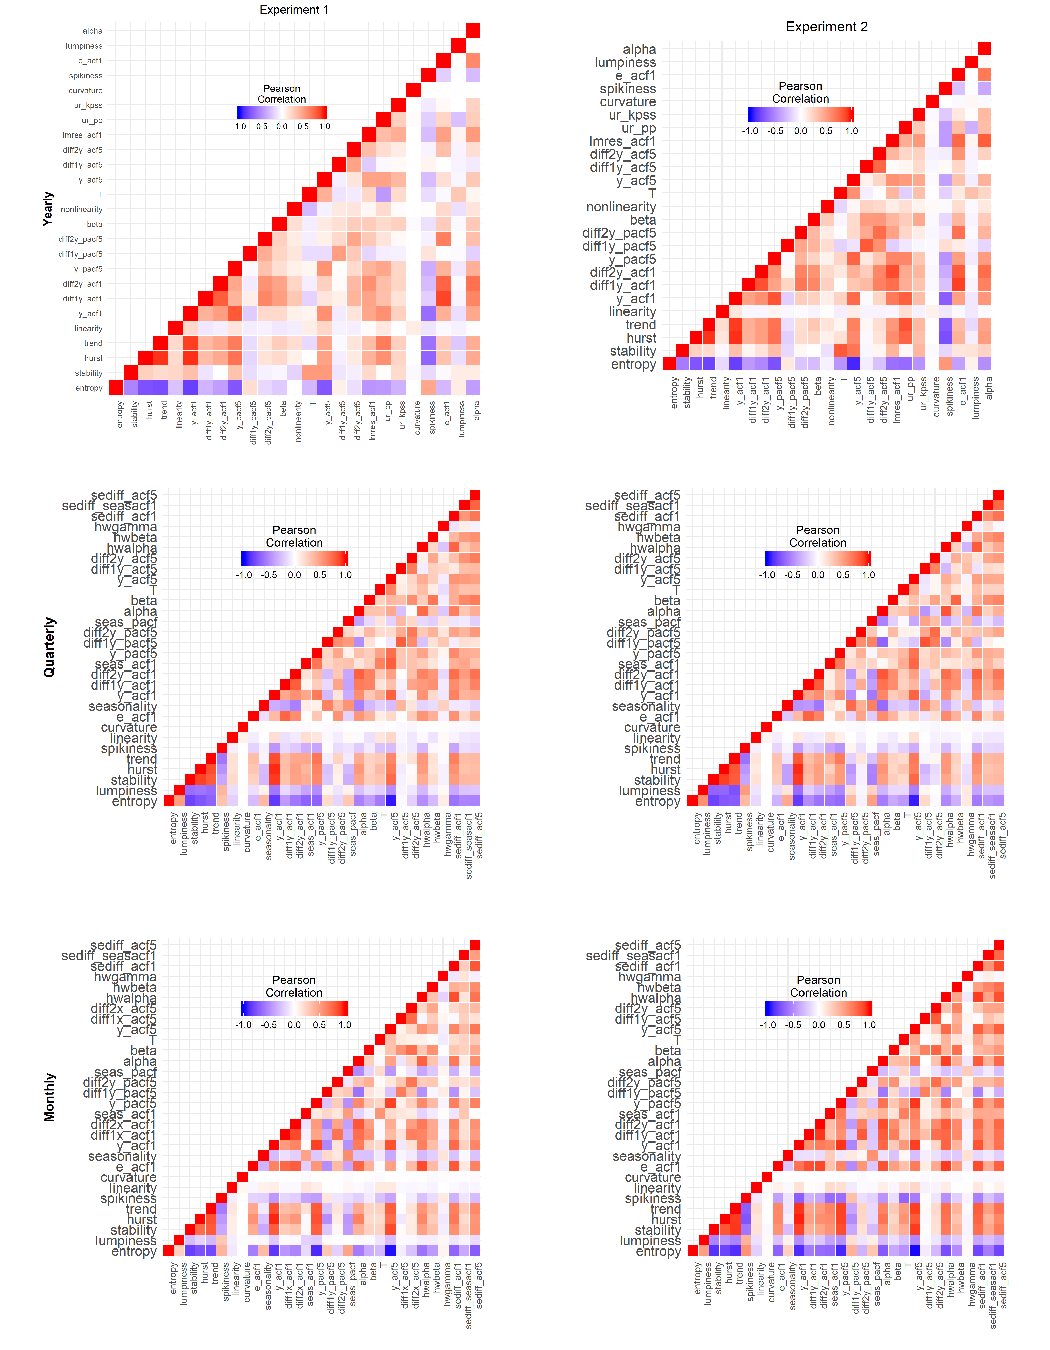
\includegraphics[width=\textwidth]{figure/cormat-1} 

}

\caption{ Correlation matrix plots for the reference sets. A: Experiment 1 yearly, B: Experiment 2 yearly, C: Experiment 1 quarterly, D: Experiment 2 quarterly, E: Experiment 1 monthly, F: Experiment 2 monthly.}\label{fig:cormat}
\end{figure}

\subsection{Model calibration}\label{model-calibration}

The random forest algorithm is highly sensitive to class imbalance
\autocite{breiman2001random}, and our reference set is unbalanced: some
classes contain significantly more cases than other classes. The degree
of class imbalance is reduced to some extent by augmenting the observed
sample with the simulated time series. We consider three approaches to
address the class imbalance in the data: 1) we incorporate class priors
into the random forest classifier; 2) we use the Balanced Random Forest
(BRF) algorithm introduced by \textcite{chen2004using}; and 3) we
re-balance the reference set with down-sampling. In down-sampling, the
size of the reference set is reduced by down-sampling the larger classes
so that they match the smallest class in size; this potentially discards
some useful information. We compare the results of these three
approaches to the classifier built on unbalanced data. The BRF and RF
with down-sampling did not yield satisfactory results. Therefore, we
reported only the results obtained by RF bulilt on unbalanced data and
RF with class priors. The RF algorithms are implemented by the
randomForest R package \autocites{liaw2002randomforest}{rfpkg}. The
class priors are introduced through the option \texttt{classwt}. We use
the reciprocal of class size as the class priors. The number of trees
\texttt{ntree} is set to 1000, and the number of randomly selected
features \texttt{mtry} is set to be one third of the total number of
features available.

Our aim is different from most classification problems in that we are
not interested in accurately predicting the class, but in finding a good
forecast-model. It is possible that two models produce almost equally
good forecasts, and then it does not matter whether the classifier picks
one or the other. Consequently, we do not study the classification
accuracy of our random forests, but only report the forecast accuracy
obtained with using them.

\subsection{Summary of the main results}\label{sec:results}

We build separate random forest classifiers for yearly data, quarterly
data and monthly data. For the second experiment, in the case of yearly
and quarterly data we take a subset of the simulated time series when
training the RF-unbalanced and RF-class priors, to reduce the size of
the reference set. The subsets are selected randomly according to the
proportions of output-labels in the observed samples. This ensures that
our reference set shares similar characteristics to the observed sample.

Principal component analysis is used to visualize the feature-spaces of
the different time series collections. We compute the principal
components projection using the features in the observed sample, and
then project the simulated time series and the new time series using the
same projection. The results are shown in Figures
\ref{fig:exp1}--\ref{fig:exp2}, where the first three principal
components are plotted against each other. Figure \ref{fig:exp1} refer
to Experiment 1 (for which M1 is the observed times series and M3 is the
new times series) and the Figure \ref{fig:exp2} to Experiment 2 (for
which M3 is the observed time series and M1 is the new time series). The
points on each plot represent individual time series. On each figure the
top three rows refer to the yearly data, the middle three to the
quarterly data and the bottom three to the monthly data. The first three
principle components explain 62.5\%, 62.4\% and 58.93\% of the total
variation in the yearly, quarterly and monthly M1 data and 62.2\%
64.75\% and 65.97\% of the total variation in the yearly, quarterly and
monthly M3 data.

The plots show that the distribution of the observed times series over
the PCA space (represented by the black dots) is very similar to that of
the new time series (represented by the orange dots). More importantly,
we see that the distribution of the simulated time series (represented
by the green dots and yellow dots - the yellow dots are a subset of the
simulated series) clearly nests that and fills in the space of the new
time series. Further, in both experiments, all the \emph{observed time
series} fall within the space of all simulated data. This strongly
indicates that we have not reduced the feature diversity from the
observed sample. This shows that our approach of augmenting the observed
time series with simulated is successful. By augmenting the reference
set with simulated time series, we were able to increase the diversity
and evenness of the feature space of the observed time series.

The accuracy of our method is compared against the following
commonly-used forecasting methods:

\begin{enumerate}
\def\labelenumi{\arabic{enumi}.}
\tightlist
\item
  automated ARIMA algorithm of \textcite{Hyndman2008};
\item
  automated ETS algorithm of \textcite{Hyndman2008};
\item
  Random walk with drift (RWD);
\item
  Random walk model (RW);
\item
  White noise process (WN);
\item
  Theta method;
\item
  STL-AR method;
\item
  seasonal naive (for seasonal data).
\end{enumerate}

The automated ARIMA and ETS algorithms are implemented using the
\texttt{auto.arima} and \texttt{ets} functions available in the forecast
package in R \autocite{forecast}. Each method is implemented on the
training period and forecasts are computed up to the full length of the
test period. Then we compute the MASE for each forecast horizon, by
averaging the MASE across all series in the collection of new time
series. To assist in the evaluation of the proposed framework, for each
forecast horizon we rank our method compared to the other methods listed
above, and an average ranking over all forecast horizons is computed.
The results are given in Table \ref{masetab}. The MASE value
corresponding to the best performing method in each category is
highlighted in bold.

\begin{figure}

{\centering 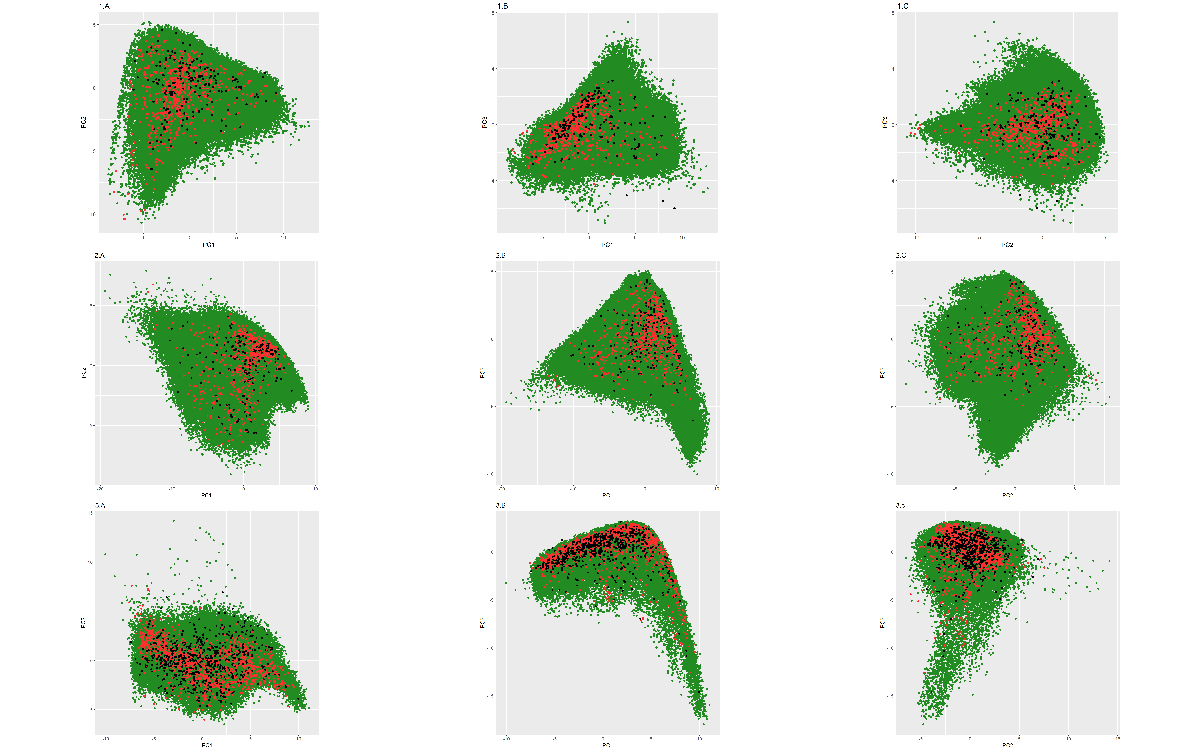
\includegraphics[width=\textwidth]{figure/exp1-1} 

}

\caption{Experiment 1: Distribution of time series in the PCA space. Distribution of yearly series are shown in panels 1A-- 1C, distribution of quarterly series are shown in panels 2A--2C, and the distribution of monthly series are shown in panels 3A--3C. On each graph, green indicates simulated time series, black indicates observed time series, while orange denotes new time series.}\label{fig:exp1}
\end{figure}

\begin{figure}

{\centering 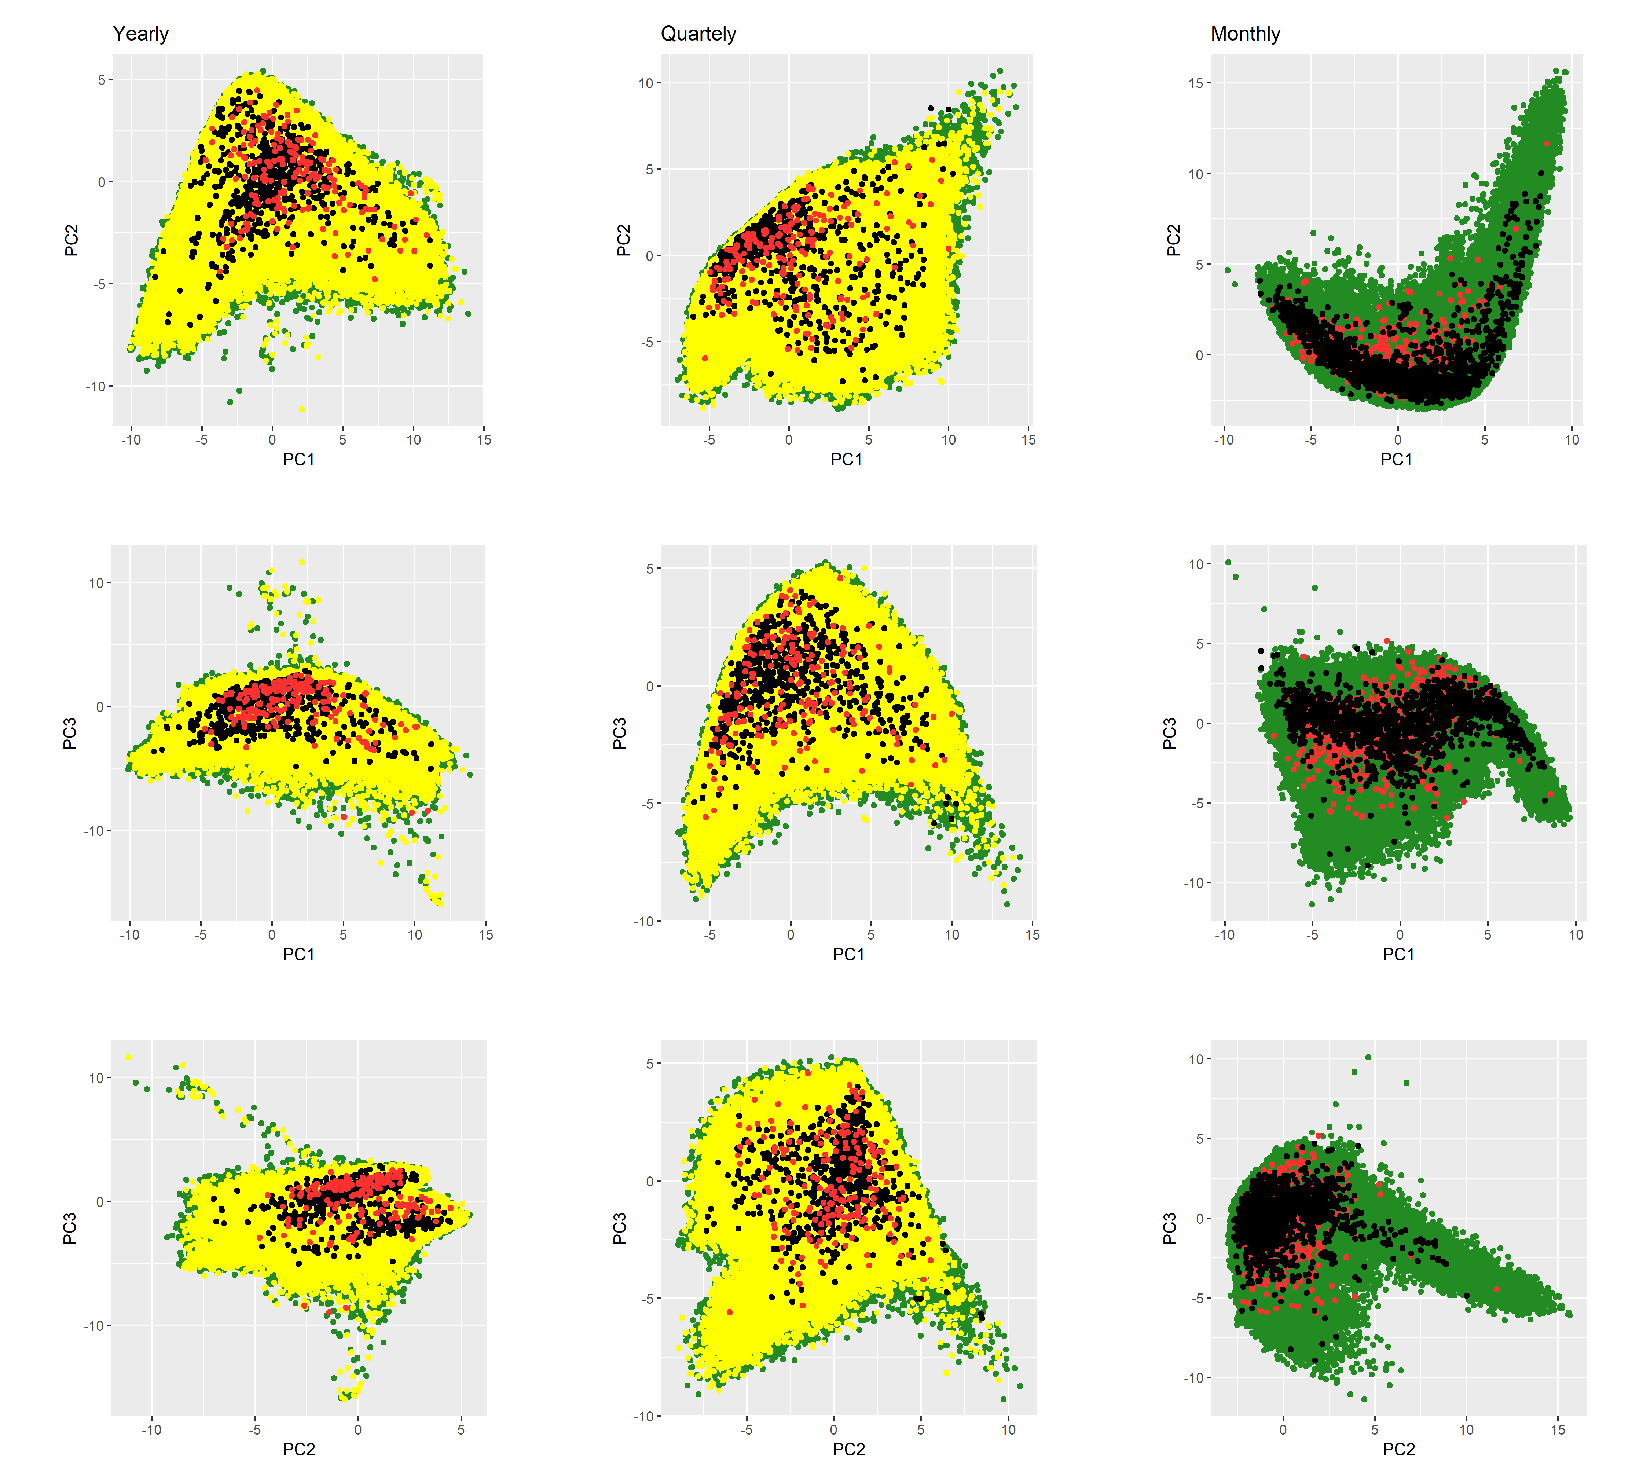
\includegraphics[width=\textwidth]{figure/exp2-1} 

}

\caption{Experiment 2: Distribution of time series in the PCA space. Distribution of yearly series are shown in panels 1A-- 1C, distribution of quarterly series are shown in panels 2A--2C, and the distribution of monthly series are shown in panels 3A--3C. On each graph, green indicates simulated time series, yellow shows a subset of simulated time series, black indicates observed time series, while orange denotes new time series.}\label{fig:exp2}
\end{figure}

\begin{table}[!htbp]
\centering\tiny
\centering
\caption{Out-of-sample forecast performances from experiment 1 and experiment 2}
\label{masetab}
\begin{tabular}{lrrrrrrcrrrrrrc}
\hline
 & \multicolumn{7}{c}{Experiment 1: training-M1, test-M3} & \multicolumn{7}{c}{Experiment 2: training-M3, test-M1} \\ \cmidrule(lr){2-8} \cmidrule(lr){9-15}
 & \multicolumn{7}{c}{Yearly: 645 M3 time series} & \multicolumn{7}{c}{Yearly: 181 M1 time series} \\ 
 & h=1  & 1-2  &  1-3 & 1-4 & 1-5 & 1-6 & avg. Rank &  h=1 & 1-2  &  1-3 & 1-4 & 1-5 & 1-6 & avg. Rank\\ \cmidrule(lr){2-8} \cmidrule(lr){9-15}
RF-unbalanced &  1.06 & 1.42  & 1.83  & 2.20 &  2.54&2.85  &  3.50& \bf{0.97}  & \bf{1.39}  & 1.93  &2.42  &  2.90& 3.37 &1.67  \\ 
RF-class priors & \bf{1.03}  & 1.37  &  1.78 &  2.14& 2.47 &  2.77&  1.83&  1.02 &  1.40 &  \bf{1.92} & \bf{2.40} & \bf{2.87} & \bf{3.33} & 1.33 \\ 
auto.arima &  1.11 &  1.48 &  1.90 &  2.28& 2.63 &2.96  & 6.83 &  1.06 &  1.47 &  2.01 &  2.51&3.00  &3.47  & 3.50 \\ 
ets & 1.09  & 1.44  & 1.84  & 2.20 &  2.54& 2.86 &  4.17& 1.12  & 1.59
&2.17   &2.72  &3.26  & 3.77 &  6.00\\ 
WN &  6.54 &  6.91 &  7.22 &  7.48& 7.76 &8.07  &9.00  &  6.38 &  7.08 &  7.92 &8.59  &9.28  &  10.01&  9.00\\ 
RW & 1.24  &  1.68 &  2.11 &  2.48& 2.83 &  3.17&8.00  &  1.35 &  2.00 &  2.80 &  3.50& 4.19 &  4.89& 8.00 \\ 
RWD & \bf{1.03}  &  \bf{1.36} & \bf{1.74}  &  \bf{2.05}&  \bf{2.35}&  \bf{2.63}&1.17  & 1.03  &  1.44 & 2.00  & 2.51 &  3.01& 3.49 &  3.33\\ 
STL-AR & 1.09  &  1.47 &  1.89 &  2.27& 2.62 &  2.95& 5.50 & 1.10  &  1.51 &  2.07 &  2.55& 3.04 & 3.52 & 5.00 \\ 
Theta & 1.12  & 1.47  & 1.86  & 2.18 &  2.48&  2.77&  4.17& 1.15  & 1.70  & 2.38  & 3.00 &  3.59& 4.19 &  7.00\\ \cmidrule(lr){2-8} \cmidrule(lr){9-15}
 & \multicolumn{7}{c}{Quarterly: 756 M3 time series} & \multicolumn{7}{c}{Quarterly: 203 M1 time series} \\ 
  & h=1  & 1-4  &  1-5 & 1-6 & 1-7 & 1-8 & avg. Rank &  h=1 & 1-4  &  1-5 & 1-6 & 1-7 & 1-8 & avg. Rank\\ \cmidrule(lr){2-8} \cmidrule(lr){9-15}
RF-unbalanced  &  0.58 &  \bf{0.81} & \bf{0.88}  &  \bf{0.96}&\bf{1.04}  &1.12  &  1.33 & \bf{0.77}  & \bf{1.08}  & \bf{1.22}  &  \bf{1.36}&  \bf{1.48}&\bf{1.59}  &  1.00\\ 
RF-class priors & 0.58  & 0.81  & 0.89  & 0.97 &  1.05&1.13  & 2.17 &  0.79 & 1.12  & 1.28& 1.41 & 1.53 & 1.65  & 2.33 \\ 
auto.arima & 0.58  & 0.85  &  0.93 & 1.01 & 1.10 & 1.19 & 4.50 &  0.85 &  1.19 & 1.37  & 1.53 &  1.67 & 1.80 & 5.00 \\ 
ets & \bf{0.56}  &  0.82 &  0.91 &  0.99& 1.08 &  1.17& 3.33 & 0.78  &  1.11 &  1.28 &  1.42& 1.54 &  1.66& 2.50 \\ 
WN  & 3.25  & 3.59  & 3.63  & 3.70 &  3.78& 3.87 &10.00  &  3.97 &  4.27 &  4.35 &  4.45& 4.52 &4.64  &  10.00\\ 
RW  & 1.14  & 1.16  & 1.25  & 1.32 &  1.41& 1.46 &7.17  &0.97   & 1.35  & 1.52  & 1.67 &  1.83& 1.95 & 7.17 \\ 
RWD & 1.20  & 1.17  &1.29   & 1.36 &  1.44& 1.47 &8.17  &0.95   & 1.26  &1.42   &1.56  &  1.71& 1.81 &  6.00\\ 
STL-AR &  0.70 &  1.27 &  1.44 &  1.60& 1.75 &  1.91& 8.50 &  0.96 &  1.63 &  1.85 &  2.05& 2.23 & 2.43 & 8.67 \\ 
Theta &  0.62 & 0.83  & 0.90  & 0.97 &  1.04& \bf{1.11} & 2.67 & 0.79  &  1.13 &  1.29 &1.42  &1.55  & 1.67 & 3.67 \\ 
Snaive & 1.11  &  1.09 &  1.21 &  1.30&  1.36&  1.43& 6.17 &  1.52 &  1.56 &  1.74 &  1.86& 1.98 &2.08  & 8.17 \\ \cmidrule(lr){2-8} \cmidrule(lr){9-15}
 & \multicolumn{7}{c}{Monthly: 1428 M3 time series} & \multicolumn{7}{c}{Monthly: 617 M1 time series} \\ 
  & h=1-4  & 1-6  &  1-8 & 1-10 & 1-12 & 1-18 & avg. Rank &  h=1-4 & 1-6  &  1-8 & 1-10 & 1-12 & 1-18 & avg. Rank\\ \cmidrule(lr){2-8} \cmidrule(lr){9-15}
RF-unbalanced &  0.66 & 0.69  & 0.72  & 0.75 &  0.75& 0.78 &  5.17& 0.72  & 0.78  & 0.83  & 0.88 &  \bf{0.89}&\bf{0.97}  &  2.50\\ 
RF-class priors & 0.65  & 0.68  & 0.71  & 0.74 &  \bf{0.74}&  \bf{0.77}&  4.00& 0.71  & 0.78  & 0.83  & 0.89 &  0.91& 0.99 &  2.83\\ 
auto.arima &  0.61 &  0.65 &  0.69 &  0.72& 0.75 &0.88  & 2.67 &0.73   &0.81   &  0.87 &  0.94& 0.99 & 1.16 & 6.83 \\ 
ets & \bf{0.59}  &  \bf{0.64} &  \bf{0.68} &  \bf{0.72}&\bf{0.74}  &  0.86&1.67  &  0.68 & 0.76  &0.82   & 0.88 & 0.93 &1.07  & 2.50 \\ 
WN &  2.06 &  2.08 &  2.10 &  2.13& 2.15 &  2.27& 12.00 & 2.06  & 2.09  & 2.12  & 2.14 &  2.18&  2.28&  12.00\\ 
RW & 0.91  &  0.97 &  1.01 &  1.04&  1.04&  1.17& 10.33 & 1.18  & 1.24  & 1.31  & 1.34 &  1.33& 1.47 & 10.00 \\ 
RWD & 0.90  & 0.96  & 1.00  & 1.03 &  1.02& 1.14 &9.17  &  1.19 & 1.27  & 1.37  &1.40  &  1.39& 1.55 & 11.00 \\ 
STL-AR &  0.73 &  0.81 &  0.90 &  0.98& 1.04 &  1.27& 8.83 &0.79   &  0.91 &  0.99 &  1.09& 1.17 & 1.39 & 8.33 \\ 
Theta & 0.63  & 0.67  & 0.72  & 0.75 &  0.77& 0.89 &  5.67& \bf{0.68}  &  \bf{0.75} & \bf{0.81}  & \bf{0.87} &  0.91& 1.04 &  1.67\\ 
Snaive &  0.95 &  0.97 &  0.97 &  0.98& 0.98 &  1.14& 9.00 &1.09   &  1.11 &  1.11 &  1.13& 1.14 & 1.31 & 8.67 \\ \hline
\end{tabular}
\end{table}

Table \ref{masetab} compare the performance of our proposed framework to
the benchmark methods. For each method, we calculate out-of-sample MASE
over the forecast horizons, and average over all time series.

For yearly series from the M3 competition, our meta-learning method
beats all methods other than the random walk with drift model. For
yearly series from the M1 competition data, our meta-learning method
using RF-unbalanced and RF-class priors consistently forecast more
accurately than all benchmark methods. For quarterly data our method
using RF-unbalanced outperforms all the bennchmark methods. For monthly
data, Table \ref{masetab} shows that our meta-learning method with
RF-unbalanced and RF-class priors provides more accurate forecasts than
the benchmark methods for the longest forecast horizons (1--18).
However, over shorter horizons, ETS does slightly better for the M3
data, and Theta does slightly better for the M1 data.

\section{Discussion and Conclusions}\label{discussion}

In this paper we have proposed a novel framework for forecast-model
selection using meta-learning based on time series features. Our
algorithm uses the knowledge of the past performance of different
forecast-models on a collection of time series in order to identify the
best forecasting method for a new series. We have shown that the method
almost always performs better than common benchmark methods, and better
than the best-performing methods from the M3 competition. Although we
have illustrated the method using the M1 and M3 competition data, the
framework is general and can be applied to any large collection of time
series.

A major advantage of our method is that it is not necessary to estimate
several different models for the data and undertake an empirical
evaluation of their forecast accuracy on a given time series. Instead,
we simply compute a small set of features that can be used to identify
the best forecasting method.

It would be possible to obtain more accurate forecasts than those we
report by combining the forecasts of many methods. However, this would
not satisfy our aim of rapid automatic forecasting, because of the
additional optimization that would be required to fit each model.

In addition to our new model selection framework, we have also
introduced a simple set of time series features that are useful in
identifying the ``best'' forecast method of a given time series, and can
be computed rapidly. We will leave to a later study an analysis of which
of these features are the most useful, and how our feature set could
reduced further without loss of forecast accuracy.

We have not compared the computation time between our method and the
benchmark methods. However, for real-time forecasting, our framework
involves only the calculation of features, the selection of a forecast
method based on the random forest classifier, and the calculation of the
forecasts from the chosen model. None of these steps involve substantial
computation and can be easily parallelised when forecasting for a large
number of new time series. For future work, we will explore the use of
other classification algorithms, and test our approach on several other
large collections of time series.

\newpage

\section*{Appendix: Definition of
features}\label{appendix-definition-of-features}
\addcontentsline{toc}{section}{Appendix: Definition of features}

\subsubsection*{Length of time series}\label{length-of-time-series}
\addcontentsline{toc}{subsubsection}{Length of time series}

The appropriate forecast-method for a time series depends on how many
observations are available. For example, shorter series tend to need
simple models such as random walk, naive method. On the other hand, for
longer time series, we have enough information to be able to estimate a
number of parameters. For even longer series (over 200 observations),
models with time-varying parameters give good forecasts as they help to
capture the inner structural changes of the model.

\subsubsection*{Features based on an
STL-decomposition}\label{features-based-on-an-stl-decomposition}
\addcontentsline{toc}{subsubsection}{Features based on an
STL-decomposition}

The strength of trend, strength of seasonality, linearity, curvature,
spikiness and first autocorrelation coefficient of the remainder series,
are calculated based on a decomposition of the time series. Suppose we
denote our time series as \(y_1, y_2, \dots,y_T\). First, a Box-Cox
transformation is applied to the time series in order to to stabilize
the variance and to make the seasonal effect additive. The transformed
series is denoted by \(y_{t}^*\). For quarterly and monthly data, this
is decomposed using STL \autocite{cleveland1990stl} to give
\(y_t^*=T_t+S_t+E_t\), where \(T_t\) denotes the trend, \(S_t\) denotes
the seasonal component, and \(E_t\) is the remainder component. For
non-seasonal data, Friedman's supersmoother \autocite{supsmu} is used to
decompose \(y_t^*=T_t+E_t\), and \(S_t=0\) for all \(t\). The detrended
series is \(x_t=y_t^*-T_t\), the deseasonalized series is
\(z_t=y_t^*-S_t\), and the remainder series is \(r_t=y_t^*-T_t-S_t\).

The strength of trend is measured by comparing the variance of the
detrended series and the original series \autocite{wang2009rule}: \[
    \text{Trend} = \text{max}\left[0, 1 - \var(r_{t})/\var(z_{t})\right].
\] Similarly, the strength of seasonality is computed as \[
    \text{Seasonality} = \text{max}\left[0, 1- \var(r_{t})/ \var(x_{t})\right].
\]

The linearity and curvature features are based on the coefficients of a
quadratic regression \[
  T_t=\beta_0+\beta_1 t + \beta_2t^2+\epsilon_t,
\] where \(t=1, 2, \dots,T\). The estimated value of \(\beta_1\) is used
as a measure of linearity while the estimated value of \(\beta_2\) is
considered as a measure of curvature. These features were used by
\textcite{hyndman2015large}.

The spikiness feature is useful when a time series is affected by
occasional outliers. \textcite{hyndman2015large} introduced an index to
measure spikiness, computed as the variance of the leave-one-out
variances of \(E_t\).

We compute the first autocorrelation coefficient of the remainder
series, \(E_t\).

\subsubsection*{Stability and lumpiness}\label{stability-and-lumpiness}
\addcontentsline{toc}{subsubsection}{Stability and lumpiness}

The features ``stability'' and ``lumpiness'' are calculated based on
tiled windows (i.e., they do not overlap). For each window, the sample
mean and variance are calculated. The stability feature is calculated as
the variance of the means, while lumpiness is the variance of the
variances. These were first used by \textcite{hyndman2015large}.

\subsubsection*{Spectral entropy of a time
series}\label{spectral-entropy-of-a-time-series}
\addcontentsline{toc}{subsubsection}{Spectral entropy of a time series}

Spectral entropy is based on information theory, and can be used as a
measure of the forecastability of a time series. Series that are easy to
forecast should have a small spectral entropy value, while very noisy
series will have a large spectral entropy. We use the measure introduced
by \textcite{goerg2013forecastable} to estimate the spectral entropy. It
estimates the Shannon entropy of the spectral density of the normalized
spectral density, given by \[ 
  H_{s}(y_t):=-\int_{-\pi}^{\pi}\hat f_y(\lambda)\log \hat f_y({\lambda})d\lambda,
\] where \(\hat{f}_y\) denotes the estimate of the spectral density
introduced by \textcite{nuttall1982spectral}. The R package ForeCA
\autocite{Foreca} was used to compute this measure.

\subsubsection*{Hurst exponent}\label{hurst-exponent}
\addcontentsline{toc}{subsubsection}{Hurst exponent}

The Hurst exponent measures the long-term memory of a time series. The
Hurst exponent is given by \(H=d+0.5\), where \(d\) is the fractal
dimension obtained by estimating a ARFIMA(\(0, d, 0\)) model. We compute
this using the maximum likelihood method \autocite{haslett1989space} as
implemented in the fracdiff package \autocite{fracdiff}. This measure
was also used in \textcite{wang2009rule}.

\subsubsection*{Nonlinearity}\label{nonlinearity}
\addcontentsline{toc}{subsubsection}{Nonlinearity}

To measure the degree of nonlinearity of the time series, we use
statistic computed in Teräsvirta's neural network test for nonlinearity
\autocite{nonlintest}, also used in \textcite{wang2009rule}. This takes
large values when the series is nonlinear, and values around 0 when the
series is linear.

\subsubsection*{Parameter estimates of an ETS
model}\label{parameter-estimates-of-an-ets-model}
\addcontentsline{toc}{subsubsection}{Parameter estimates of an ETS
model}

The ETS(A,A,N) model \autocite{expsmooth08} produces equivalent
forecasts to Holt's linear trend method, and can be expressed as
follows:\vspace*{-.9cm}

\begin{align*}
  y_t    & = \ell_{t-1}+b_{t-1}+\varepsilon_t\\
  \ell_t & = \ell_{t-1}+b_{t-1}+\alpha \varepsilon_t\\
  b_t    & = b_{t-1}+\beta \varepsilon_t,\vspace*{-0.99cm}
\end{align*}

where \(\alpha\) is the smoothing parameter for the level, and \(\beta\)
is the smoothing parameter for the trend. We include the parameter
estimates of both \(\alpha\) and \(\beta\) in our feature set for yearly
time series.

The ETS(A,A,N) model \autocite{expsmooth08} produces equivalent
forecasts to Holt-Winters' additive method, and can be expressed as
follows:\vspace*{-.9cm}

\begin{align*}
  y_t    & = \ell_{t-1}+b_{t-1}+s_{t-m}+\varepsilon_t\\
  \ell_t & = \ell_{t-1}+b_{t-1}+s_{t-m}+\alpha \varepsilon_t\\
  b_t    & = b_{t-1}+\beta \varepsilon_t,\\
  s_t &= s_{t-m} + \gamma\varepsilon_t,\vspace*{-0.99cm}
\end{align*}

where \(\gamma\) is the smoothing parameter for the seasonal component,
and the other parameters are as above. We include the parameter
estimates of \(\alpha\), \(\beta\) and \(\gamma\) in our feature set for
monthly and quarterly time series.

\subsubsection*{Unit root test
statistics}\label{unit-root-test-statistics}
\addcontentsline{toc}{subsubsection}{Unit root test statistics}

The Phillips-Perron test is based on the regression
\(y_t=\alpha+(\phi)y_{t-1}+ \epsilon_t\). The test statistic we use as a
feature is \[
  Z = T(\hat{\phi}-1)- T^2\text{se}(\hat{\phi})(\hat{\lambda}^2-\hat{\sigma^2})/2\hat\sigma^2,
\] where \(\hat\sigma^2= T^{-1}\sum_{t=1}^{T} \hat\epsilon_t^2\),
\(\hat\lambda^2=T^{-1} \sum_{t=1}^{T} S_T^2\), and
\(S_T = \sum_{t=1}^{T}\hat\epsilon_t\).

The KPSS test is based on the regression
\(y_t=c+\delta t+\phi y_{t-1}+\epsilon_t\). The test statistic we use as
a feature is \[
  Z= \hat{\sigma}^{-2} T^{-2}\sum_{t=1}^{T}S_t^2,
\] where \(S_t=\sum_{j=1}^T\hat{\epsilon}_j\), and
\(\hat{\sigma}^2 = T^{-1}\sum_{t=1}^{T} \hat\epsilon_t^2\).

Features based on unit root tests are calculated using the \texttt{urca}
package \autocite{pfaff2016package}.

\subsubsection*{Autocorrelation coefficient based
features}\label{autocorrelation-coefficient-based-features}
\addcontentsline{toc}{subsubsection}{Autocorrelation coefficient based
features}

We calculate the first-order autocorrelation coefficient and the sum of
squares of the first five autocorrelation coefficients of the original
series, the first-differenced series, the second-differenced series, and
the seasonally differenced series (for seasonal data).

A linear trend model is fitted to the time series, and the first-order
autocorrelation coefficient of the residual series is calculated.

We calculate the sum of squares of first five partial autocorrelation
coefficients of the original series, the first-differenced series and
the second-differenced series.

\newpage

\printbibliography[title=References]

\end{document}
